\let\negmedspace\undefined
\let\negthickspace\undefined
\documentclass[journal]{IEEEtran}
\usepackage[a5paper, margin =  10mm, onecolumn]{geometry}
%\usepackage{lmodern} % Ensure lmodern is loaded for pdflatex
\usepackage{tfrupee} % Include tfrupee package

\setlength{\headheight}{1cm} % Set the height of the header box
\setlength{\headsep}{0mm}     % Set the distance between the header box and the top of the text

\usepackage{gvv-book}
\usepackage{gvv}
\usepackage{cite}
\usepackage{amsmath,amssymb,amsfonts,amsthm}
\usepackage{algorithmic}
\usepackage{graphicx}
\usepackage{textcomp}
\usepackage{xcolor}
\usepackage{txfonts}
\usepackage{listings}
\usepackage{enumitem}
\usepackage{mathtools}
\usepackage{gensymb}
\usepackage{comment}
\usepackage[breaklinks =  true]{hyperref}
\usepackage{tkz-euclide} 
\usepackage{listings}
% \usepackage{gvv}                                        
\def\inputGnumericTable{}                                 
\usepackage[latin1]{inputenc}                                
\usepackage{color}                                            
\usepackage{array}                                            
\usepackage{longtable}                                       
\usepackage{calc}                                             
\usepackage{multirow}                                         
\usepackage{hhline}                                           
\usepackage{ifthen}                                           
\usepackage{lscape}
\begin{document}

\bibliographystyle{IEEEtran}
\vspace{1cm}

\title{4.11.12}
\author{EE25BTECH11034 - Kishora Karthik}
% \maketitle
% \newpage
% \bigskip
{\let\newpage\relax\maketitle}

\renewcommand{\thefigure}{\theenumi}
\renewcommand{\thetable}{\theenumi}
%\setlength{\intextsep}{10pt} % Space between text and floats
\textbf{Question:}\\
Find the distance of the point $P(-1,-5,-10)$ from the point of intersection of the line
$\vec{r} = 2\hat{\imath}-\hat{\jmath}+2\hat{k}+\lambda\,(3\hat{\imath}+4\hat{\jmath}+2\hat{k})$
and the plane
$\vec{r}\cdot(\hat{\imath}-\hat{\jmath}+\hat{k})=5$.
\\
\textbf{Solution:}\\
The line is given by $\vec{x}=\vec{h}+k\vec{m}$, where 
\begin{align}
    \vec{x}=\myvec{2\\-1\\2}
\end{align}
\begin{align}
    \vec{m}=\myvec{3\\4\\2}
\end{align}
The plane is of the form $\vec{n}^\top\vec{x}=c$ where $c=5$ and,
\begin{align}
\vec{n}=\myvec{1\\-1\\1}
\end{align}
Given, $\vec{P}=\myvec{-1\\-5\\-10}$.
To find the point of intersection, we substitute the vector equation of the line into the vector equation of the plane.
\begin{align}
(\vec{a} + \lambda\vec{b}) \cdot \vec{n} = c
\end{align}
\begin{align}
\vec{h} \cdot \vec{n} + k(\vec{m} \cdot \vec{n}) = c
\end{align}
\begin{align}
\vec{h}  \vec{n}^\top + k(\vec{m} \vec{n}^\top) = c
\end{align}
\begin{align}
\myvec{2\\-1\\2} \cdot \myvec{1&-1&1} + k\myvec{3\\4\\2} \cdot \myvec{1&-1&1} = 5
\end{align}
\begin{align}
(2\cdot1+(-1)\cdot(-1)+(2)\cdot(1))+k(3\cdot1+4\cdot(-1)+2\cdot(1)) = 5    
\end{align}
\begin{align}
    (5)+k(1) = 5
\end{align}
\begin{align}
    k = 0
\end{align}
The point of intersection is $\vec{x} = \vec{h} + 0(\vec{m}) = \vec{h} $.
\\Distance between two points is given by 
$\norm{\vec{x_2}-\vec{x_1}}$.\\
\begin{align}
    d=\norm{\myvec{-1\\-5\\-10}-\myvec{2\\-1\\2}}
\end{align}
\begin{align}
    d=\norm{\myvec{-3\\-4\\12}}
\end{align}
\begin{align}
    d=\sqrt{(-3)^2+(-4)^2+(12)^2}
\end{align}
\begin{align}
    d=\sqrt{169}
\end{align}
\begin{align}
    d=13
\end{align}
$\therefore$ The distance between the points is 13 units.
\centering   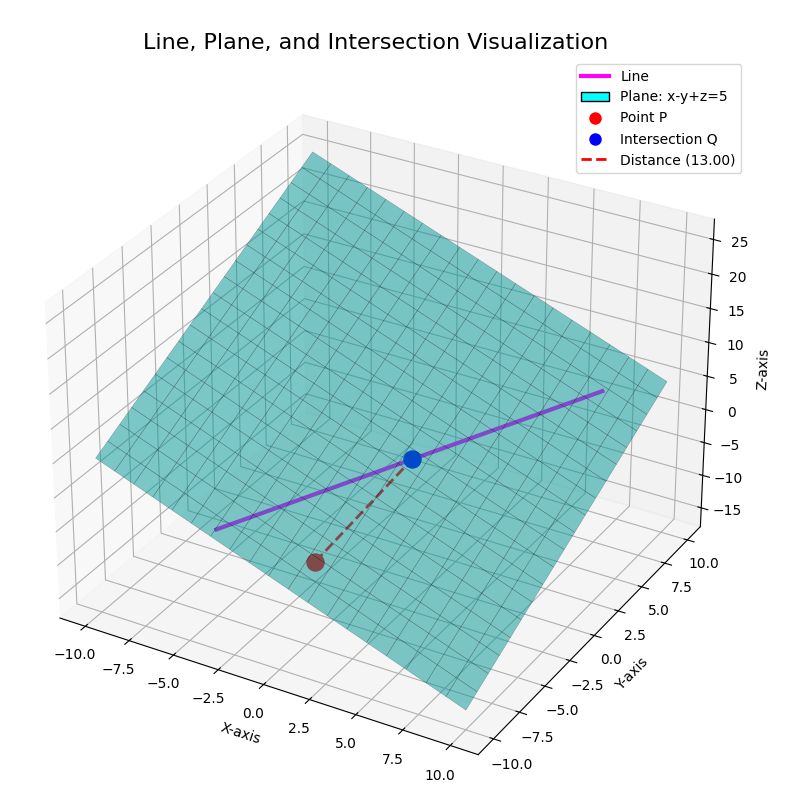
\includegraphics[width=\columnwidth, height=\textheight, keepaspectratio]{figs/fig1.png}
\end{document}
